\documentclass[border=6pt]{standalone}
\usepackage{amsmath}
\usepackage{tikz}
\usetikzlibrary{arrows.meta}
\begin{document}
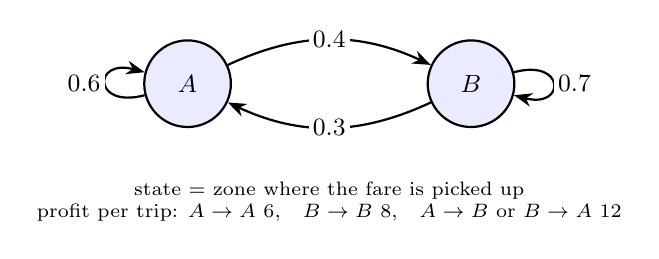
\begin{tikzpicture}[>=Stealth,font=\small,
 s/.style={draw,thick,circle,minimum size=1.1cm,inner sep=0pt,fill=blue!8},
 e/.style={->,thick},
 lab/.style={font=\small,fill=white,inner sep=1.5pt},
 every loop/.style={->,thick,looseness=6}]
\node[s] (A) at (0,0) {$A$};
\node[s] (B) at (3.6,0) {$B$};
\draw[e] (A) to[bend left=25] node[lab]{0.4} (B);
\draw[e] (B) to[bend left=25] node[lab]{0.3} (A);
\path (A) edge[loop left] node[lab]{0.6} (A);
\path (B) edge[loop right] node[lab]{0.7} (B);
\node[font=\scriptsize,align=center] at (1.8,-1.5) {state = zone where the fare is picked up\\profit per trip: $A\to A$ 6,\quad $B\to B$ 8,\quad $A\to B$ or $B\to A$ 12};
\end{tikzpicture}
\end{document}
